\documentclass[aspectratio=169]{../latex_main/tntbeamer}  % you can pass all options of the beamer class, e.g., 'handout' or 'aspectratio=43'
\usepackage{dsfont}
\usepackage{bm}
\usepackage[english]{babel}
\usepackage[T1]{fontenc}
%\usepackage[utf8]{inputenc}
\usepackage{graphicx}
\graphicspath{ {./figures/} }
\usepackage{algorithm}
\usepackage[ruled,vlined,algo2e,linesnumbered]{algorithm2e}
\usepackage{hyperref}
\usepackage{booktabs}
\usepackage{mathtools}

\usepackage{amsmath,amssymb}

\DeclareMathOperator*{\argmax}{arg\,max}
\DeclareMathOperator*{\argmin}{arg\,min}

\usepackage{amsbsy}
\newcommand{\vect}[1]{\bm{#1}}
%\newcommand{\vect}[1]{\boldsymbol{#1}}

\usepackage{pgfplots}
\pgfplotsset{compat=1.16}
\usepackage{tikz}
\usetikzlibrary{trees} 
\usetikzlibrary{shapes.geometric}
\usetikzlibrary{positioning,shapes,shadows,arrows,calc,mindmap}
\usetikzlibrary{positioning,fadings,through}
\usetikzlibrary{decorations.pathreplacing}
\usetikzlibrary{intersections}
\pgfdeclarelayer{background}
\pgfdeclarelayer{foreground}
\pgfsetlayers{background,main,foreground}
\tikzstyle{activity}=[rectangle, draw=black, rounded corners, text centered, text width=8em]
\tikzstyle{data}=[rectangle, draw=black, text centered, text width=8em]
\tikzstyle{myarrow}=[->, thick, draw=black]

% Define the layers to draw the diagram
\pgfdeclarelayer{background}
\pgfdeclarelayer{foreground}
\pgfsetlayers{background,main,foreground}

% Requires XeLaTeX or LuaLaTeX
%\usepackage{unicode-math}

\usepackage{fontspec}
%\setsansfont{Arial}
\setsansfont{RotisSansSerifStd}[ 
Path=../latex_main/fonts/,
Extension = .otf,
UprightFont = *-Regular,  % or *-Light
BoldFont = *-ExtraBold,  % or *-Bold
ItalicFont = *-Italic
]
\setmonofont{Cascadia Mono}[
Scale=0.8
]

% scale factor adapted; mathrm font added (Benjamin Spitschan @TNT, 2021-06-01)
%\setmathfont[Scale=1.05]{Libertinus Math}
%\setmathrm[Scale=1.05]{Libertinus Math}

% other available math fonts are (not exhaustive)
% Latin Modern Math
% XITS Math
% Libertinus Math
% Asana Math
% Fira Math
% TeX Gyre Pagella Math
% TeX Gyre Bonum Math
% TeX Gyre Schola Math
% TeX Gyre Termes Math

% Literature References
\newcommand{\lit}[2]{\href{#2}{\footnotesize\color{black!60}[#1]}}

%%% Beamer Customization
%----------------------------------------------------------------------
% (Don't) Show sections in frame header. Options: 'sections', 'sections light', empty
\setbeamertemplate{headline}{empty}

% Add header logo for normal frames
\setheaderimage{
	% 
\includegraphics[height=\logoheight]{figures/TNT_darkv4.pdf}
	
\includegraphics[height=\logoheight]{../latex_main/figures/luh_logo_rgb_0_80_155.pdf}
	% 
\includegraphics[height=\logoheight]{figures/logo_tntluh.pdf}
}

% Header logo for title page
\settitleheaderimage{
	% 
\includegraphics[height=\logoheight]{figures/TNT_darkv4.pdf}
	
\includegraphics[height=\logoheight]{../latex_main/figures/luh_logo_rgb_0_80_155.pdf}
	% 
\includegraphics[height=\logoheight]{figures/logo_tntluh.pdf}
}

% Title page: tntdefault 
\setbeamertemplate{title page}[tntdefault]  % or luhstyle
% Add optional title image here
%\addtitlepageimagedefault{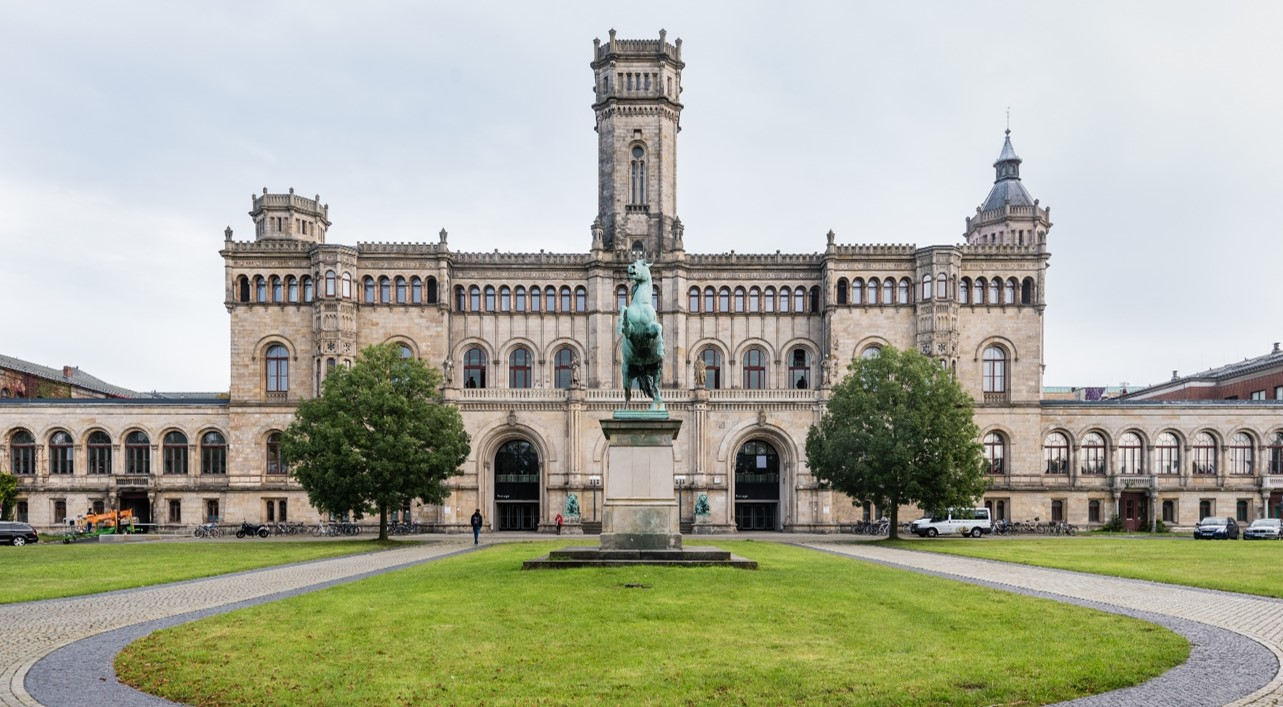
\includegraphics[width=0.65\textwidth]{figures/luh_default_presentation_title_image.jpg}}

% Title page: luhstyle
% \setbeamertemplate{title page}[luhstyle]
% % Add optional title image here
% \addtitlepageimage{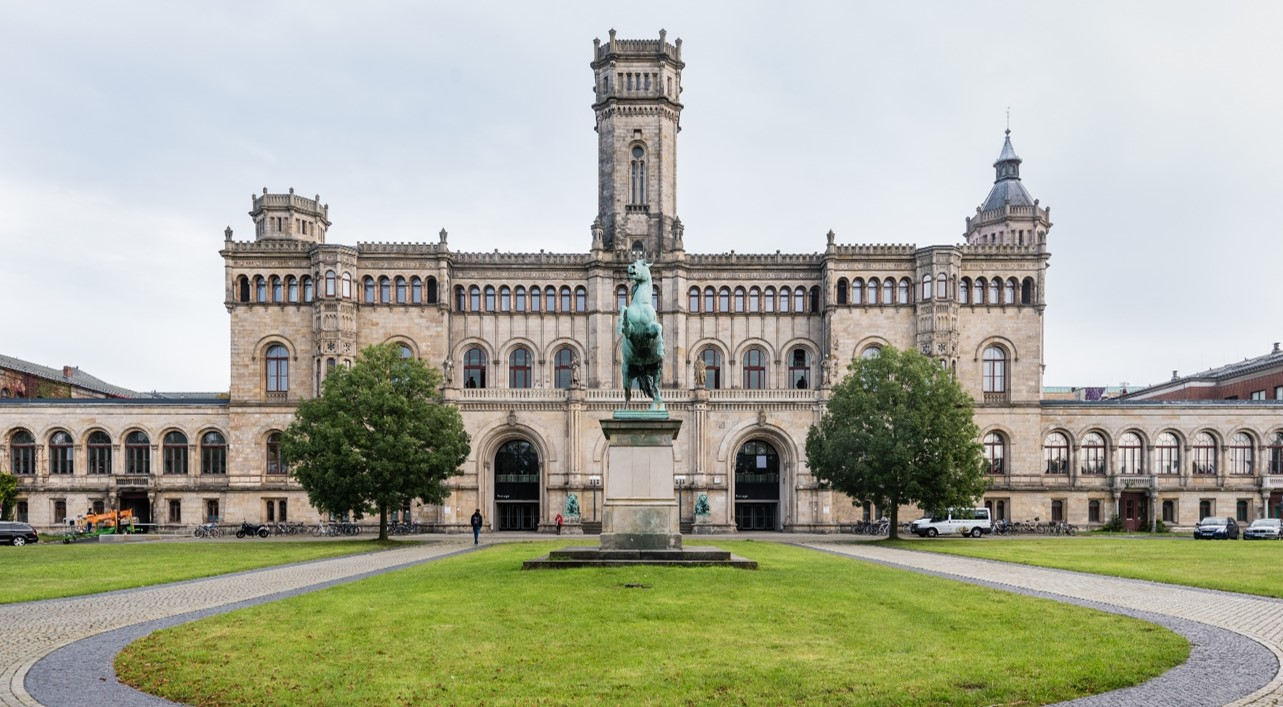
\includegraphics[width=0.75\textwidth]{figures/luh_default_presentation_title_image.jpg}}

\author[Abedjan \& Lindauer]{Ziawasch Abedjan \& Marius Lindauer\\[1em]
	
\includegraphics[height=\logoheight]{../latex_main/figures/luh_logo_rgb_0_80_155.pdf}\qquad
	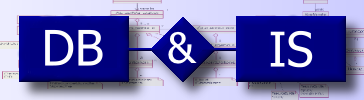
\includegraphics[height=\logoheight]{../latex_main/figures/DBIS_Kurzlogo.png}\qquad

\includegraphics[height=\logoheight]{../latex_main/figures/TNT_darkv4}\qquad

\includegraphics[height=\logoheight]{../latex_main/figures/L3S.jpg}	}
\date{Summer Term 2022; \hspace{0.5em} {
\includegraphics[height=1.5em]{../latex_main/figures/Cc-by-nc-sa_icon.svg.png}}; based on \href{https://ds100.org/fa21/}{[DS100]}
}


%%% Custom Packages
%----------------------------------------------------------------------
% Create dummy content
\usepackage{blindtext}

% Adds a frame with the current page layout. Just call \layout inside of a frame.
\usepackage{layout}


%%% Macros
%\renewcommand{\vec}[1]{\mathbf{#1}}
% \usepackage{bm}
%\let\vecb\bm

\title[Introduction]{DS: Data Cleaning and EDA}
\subtitle{File Formats and Structure}

\graphicspath{ {./figure/} }
%\institute{}


\begin{document}
	
	\maketitle
	\begin{frame}{What should we look for?}
	    
	\end{frame}
	
	
	
	\begin{frame}{Key Data Properties to Consider in EDA}
	    \begin{itemize}
	        \item Structure -- the “shape” of a data file
	        \item Granularity -- how fine/coarse is each datum
	        \item Scope -- how (in)complete is the data
	        \item Temporality -- how is the data situated in time
	        \item Faithfulness -- how well does the data capture “reality”
	    \end{itemize}
	\end{frame}
	
	
	\begin{frame}{Key Data Properties to Consider in EDA}
	    \begin{itemize}
	        \item \textbf{Structure -- the “shape” of a data file}
	        \item Granularity -- how fine/coarse is each datum
	        \item Scope -- how (in)complete is the data
	        \item Temporality -- how is the data situated in time
	        \item Faithfulness -- how well does the data capture “reality”
	    \end{itemize}
	\end{frame}
	
	
	
	\begin{frame}{Key Data Properties to Consider in EDA}
	    \begin{itemize}
	        \item \textbf{Structure -- the “shape” of a data file}
	        \item Granularity -- how fine/coarse is each datum
	        \item Scope -- how (in)complete is the data
	        \item Temporality -- how is the data situated in time
	        \item Faithfulness -- how well does the data capture “reality”
	    \end{itemize}
	\end{frame}
	
	
	
	\begin{frame}{Rectangular Data}
	   \begin{columns}
	   
	   
	   \begin{column}{.7\textwidth}
	    
	   
	    We prefer rectangular data for data analysis (why?)
	    \begin{itemize}
	        \item Regular structures are easy manipulate and analyze
	        \item A big part of data cleaning is about transforming data to be more rectangular
	    \end{itemize}
	    
        Two kinds of rectangular data: Tables and Matrices \\
		\centering	(what are the differences?)
		\end{column}
		
	   \begin{column}{.3\textwidth}
	   \begin{figure}
	       		    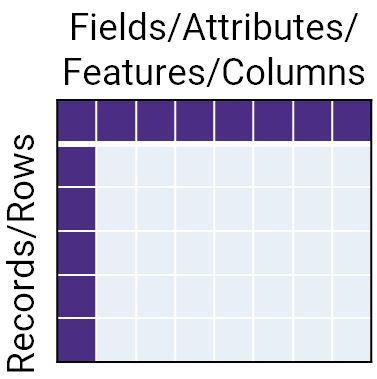
\includegraphics[scale=.3]{Bild8}
	   \end{figure}

		\end{column}
		\end{columns}
	\end{frame}
	
	
	\begin{frame}{Rectangular Data}
	   \begin{columns}
	   
	   
	   \begin{column}{.7\textwidth}
	    
	   
	    We prefer rectangular data for data analysis (why?)
	    \begin{itemize}
	        \item Regular structures are easy manipulate and analyze
	        \item A big part of data cleaning is about transforming data to be more rectangular
	    \end{itemize}
	    
        Two kinds of rectangular data: Tables and Matrices \\
		\centering	(what are the differences?)
		\end{column}
		
	   \begin{column}{.3\textwidth}
	   \begin{figure}
	       		    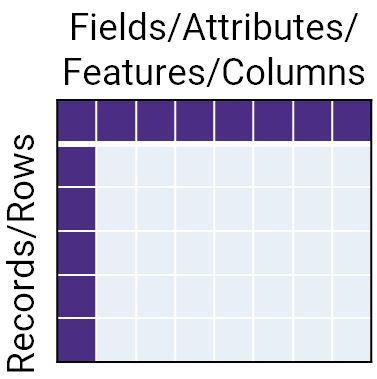
\includegraphics[scale=.3]{Bild8}
	   \end{figure}

		\end{column}
		\end{columns}
		
	\begin{itemize}
		    \item[1.] Tables (a.k.a. data-frames  in R/Python and relations in SQL)
		    \begin{itemize}
		        \item Named columns with different types
		        \item Manipulated using data transformation languages (map, filter, group by, join, …)
		    \end{itemize}
		    \item[2.] Matrices
		    \begin{itemize}
		        \item Numeric data of the same type
		        \item Manipulated using linear algebra 
		    \end{itemize}
		\end{itemize}
	\end{frame}
	
	
	
	
	\begin{frame}{How are these data files formatted?}
	    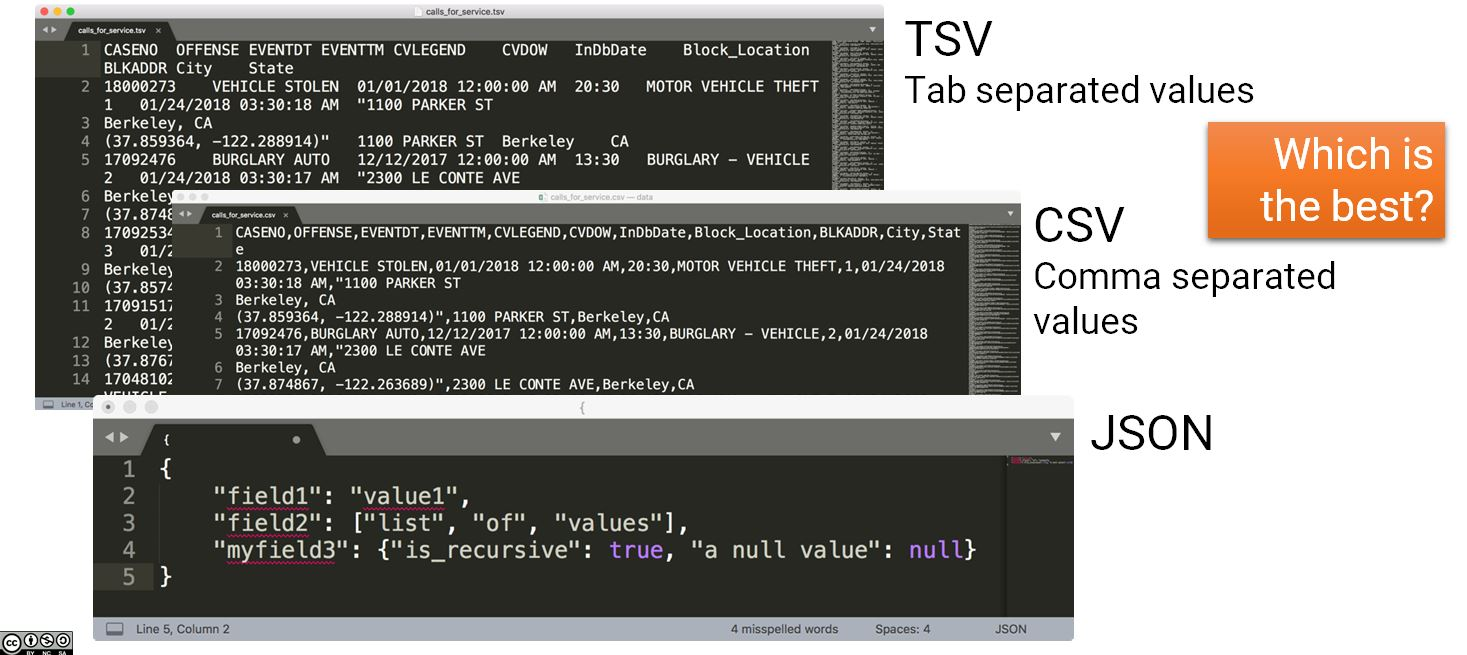
\includegraphics[scale=.39]{Bild9}
	\end{frame}



    \begin{frame}{Comma and Tab Separated Values Files}
	   \begin{columns}
	   
	   
	   \begin{column}{.4\textwidth}
	    
	    \begin{itemize}
	        \item Tabular data where
	        \begin{itemize}
	            \item Records are delimited by a newline: “\n”, “\r\n”
	            \item Fields are delimited by ‘,’ (comma) or ‘\t’ (tab)
	        \end{itemize}
	        \item Very Common! 
	        \item Issues?
	        \begin{itemize}
	            \item Commas, tabs in records
	            \item Quoting
	            \item \dots
	        \end{itemize}
	    \end{itemize}
		\end{column}
		
	   \begin{column}{.4\textwidth}
	   \begin{figure}
	       		    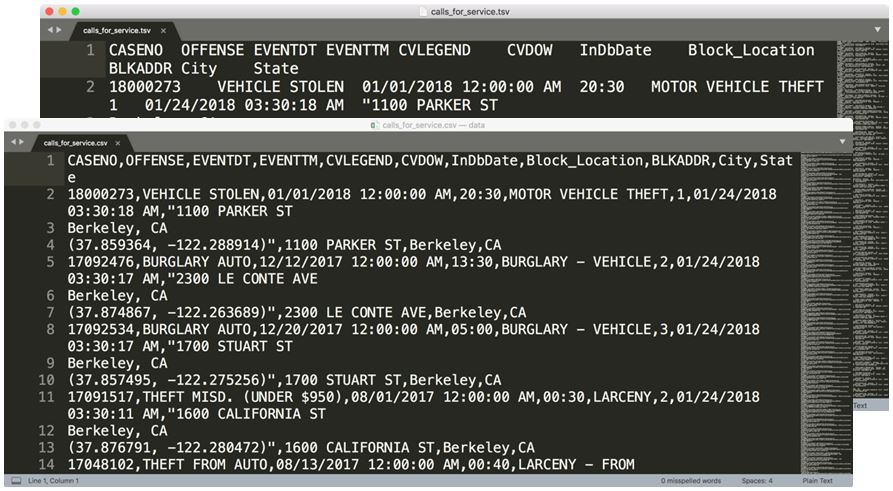
\includegraphics[scale=.3]{Bild10}
	   \end{figure}

		\end{column}
		\end{columns}
	\end{frame}
	
	
	
	\begin{frame}{JavaScript Object Notation (JSON)}
	           \centering                                                                                           
	           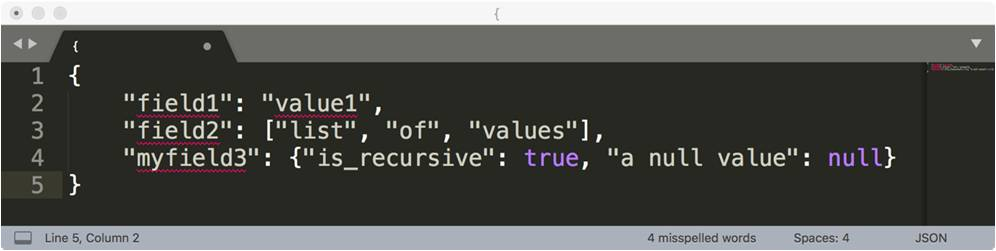
\includegraphics[scale=.75]{Bild11}                               
	   \begin{itemize}
	       \item Widely used file format for nested data
	       \begin{itemize}
	           \item Very similar to python dictionaries
	           \item Strict formatting ”quoting” addresses some issues in CSV/TSV
	       \end{itemize}
	       \item Issues
	       \begin{itemize}
	           \item Not rectangular
	           \item Each record can have different fields
	           \item Nesting means records can contain tables – complicated
	       \end{itemize}
	   \end{itemize}
	\end{frame}
	
	
	
	\begin{frame}{Extensible Markup Language - XML (another kind of nested data)}
	                                                                                      
	           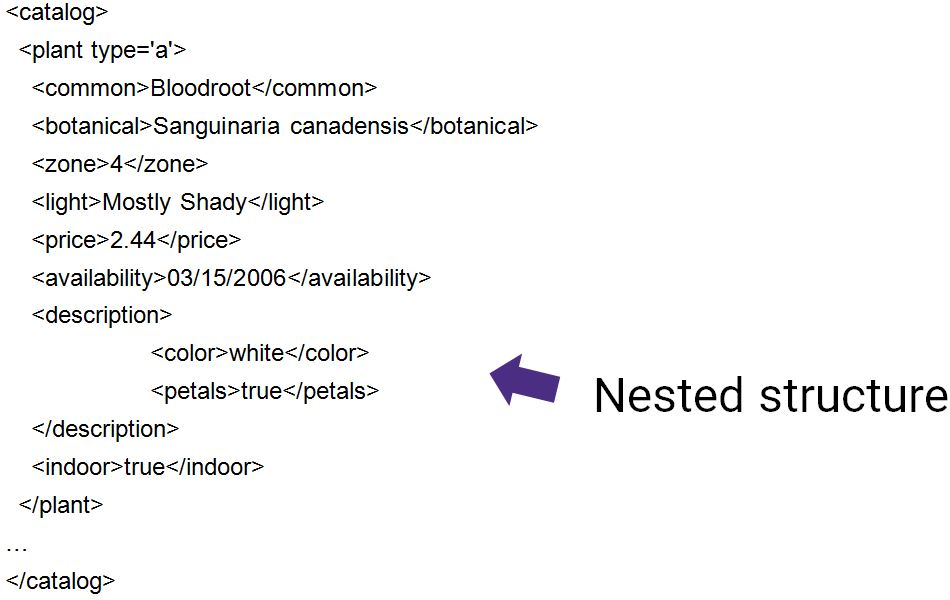
\includegraphics[scale=.4]{Bild12}                               
	\end{frame}
	
	
	
	
	\begin{frame}{Log Data}
	               Is this a csv file? tsv? JSON/XML?\\
                                                                       
	           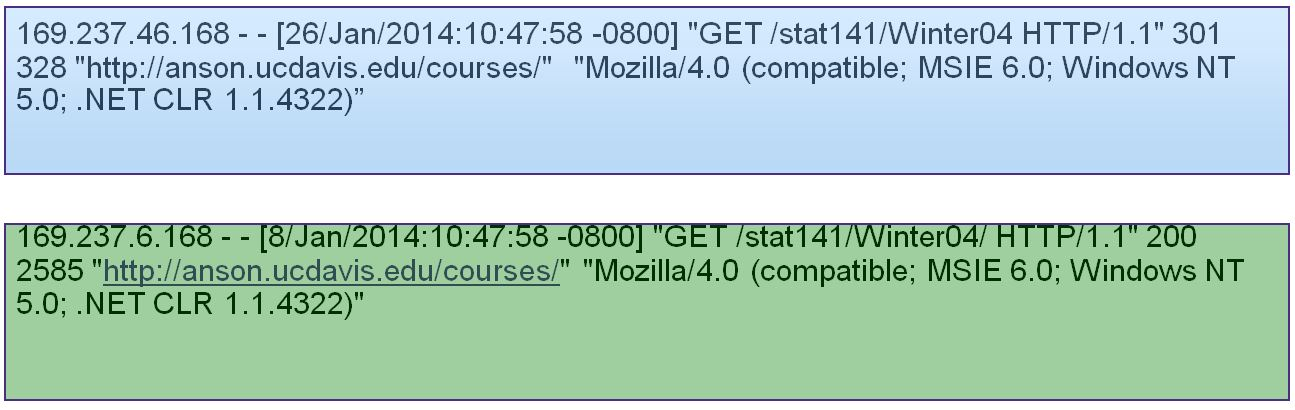
\includegraphics[scale=.4]{Bild13}                               
	\end{frame}
\end{document}